\chapter{Background}
\label{background}
Isaac Newton was the first person to consider the possibility of exoplanets
 \citep{principia}. It requires little more than a simple understanding of the
 solar system and Newtonian physics to consider the possibility that other stars
 may host their own planets. Any planet orbiting any star must obey Newton's
 version of Kepler's 3rd law,

\begin{equation}
    T^2=\frac{4\pi^2}{\mathrm{G}\left(m_{*}+m_{p}\right)}a^3,
    \label{nvktl}
\end{equation}
where $T$ is the orbital period of the orbit, $a$ is its semi-major axis, $m_*$ is
 the mass of the star, and $m_p$ is the mass of the planet. In addition, the
 small mass approximation where $m_*>>m_p$ simplifies equation \ref{nvktl} to

\begin{equation}
    T^2=\frac{4\pi^2}{\mathrm{G}m_{*}}a^3,
\end{equation}
which we can solve, even if the mass of the planet is unknown. If the orbital
 period of an exoplanet and the mass of the host star are known; the planet's
 semi-major axis can be calculated. Using the semi-major axis, the planet's
 solar irradiance can be calculated with

\begin{equation}
    S_p=\mathrm{\sigma} T_{*}^{4}\frac{r_{*}^2}{a^2},
\end{equation}
where $S_p$ is the solar irradiance for the exoplanet. This value can be
 calculated using only a few data points, and can be compared to the solar
 irradiance of Earth
 ($\mathrm{S}_{\earth}\approx1361 \si{\watt\per\meter\squared}$). A simple
 narrative would be that if the $S_{p}\approx \mathrm{S}_{\earth}$, then the
 planet is Earth-like. This understanding defined exoplanetary knowledge for
 hundreds of years, and technological limitations slowed further progress in
 our understanding of exoplanets.

The most na\"{i}ve method for detecting an exoplanet is by direct imaging, just
 like we do for stars; however, the math behind this isn't very
 promising. If you approximate a planet as a blackbody, its flux is proportional
 to $R^{2}T^{4}$, then a \SI{300}{\kelvin} exoplanet with a radius of
 $1\mathrm{R}_{\earth}$ around a \SI{3000}{\kelvin} star with a radius of
 $0.17\ R_{\sun}$ would be $\nicefrac{1}{10,000,000^\mathrm{th}}$ as bright,
 which corresponds to a difference in 16 magnitudes. While observing two stars
 16 magnitudes apart is certainly possible in optimal circumstances, it is
 virtually impossible to do when trying to view exoplanets because an exoplanet
 and its host star are almost always within the diffraction limit of each other.
 Telescopes large enough to detect an exoplanet have existed for over a hundred
 years, the primary limitation has always been the instrumentation.

This changed with the introduction of the CCD, which allowed for accurate
 photometry of dim objects in relatively short time periods.
 Astronomers are now able to detect exoplanets with a new method, instead of
 measuring the brightness of the planet, it is possible to measure the change in the
 brightness of the star. In 2003, the first exoplanet was detected by measuring
 the decrease in the star's brightness as the planet passed in front of its host
 star \citep{firsttransit}. This became known as the ``transit method,'' and to
 date, this method has detected more exoplanets than any other. The transit
 method only requires simple photometry, which can be done with significantly
 higher signal to noise than spectroscopy. Typically, transits are found using
 relative photometry; where the brightness of a star during transit is
 compared to the brightness of other stars in the field. This means that
 measurements can be accurate despite the presence of systematic errors. In a
 transit, the measured signal is the decrease in the brightness of the star
 relative to its normal brightness, so the measured value is called transit
 depth, and can be given by

\begin{equation}
    D=\frac{R_p^2}{R_*^2},
\end{equation}
where D is the transit depth, $R_p$ is the planet radius, and $R_*$ is the star
 radius. Using the above example of a 1 $\mathrm{R}_\earth$ planet around a
 $0.17\, \mathrm{R}_\sun$ star, the transit depth would be 0.0028, or
 $\nicefrac{3}{1000^\mathrm{th}}$ the brightness of the star, which can be
 measured fairly reliably. The most observable exoplanets are large planets
 around small stars. Small stars are less likely to drown out the signal of a
 planet, and large planets are likely to create larger signals. A large planet
 around a small star would have a large transit depth. Transit depth is usually
 reported in parts per million (ppm) instead of as a
 decimal, as it will for the remainder of this thesis.

Another useful method to detect exoplanets is through measuring the radial
 velocity of the host star. As an
 exoplanet orbits its host star, the star should move as well much more slowly
 than a planet. With the use of a spectrograph, the doppler shift of a host star
 can be measured. Usually a star may be moving at speeds so low, they're
 measures in centimeters per second, but it can still be measured reliably. By
 applying the laws of conservation of momentum, the relationship

\begin{equation}
    m_*v_*=m_pv_p,
\end{equation}
where $m$ represents the mass, $v$ represents the velocity, * represents the star
 and $p$ represents the planet. The star mass is known from the star's temperature
 and size, and the planet's velocity can be deduced from Kepler's laws. This
 method can be useful for measuring the masses of large planets, but the radial
 velocity methods fails when the planetary mass is too small to produce a large
 stellar velocity. This method is much easier to implement, and is therefore
 how we detected the first exoplanets \citep{firstradv}. The radial velocity method can
 often be used in conjunction with the transit method because transiting
 exoplanets will produce the strongest possible radial velocity measurements.
 For more complicated systems with multiple planets, the radial velocity method
 becomes more difficult, and other methods are more useful for measuring
 planetary mass.

Unfortunately, there are some major limitations to the transit method. The most
 scientifically interesting exoplanets are terrestrial exoplanets are approximately
 $1\,\mathrm{R}_\earth$, approximately $1\,\mathrm{m}_\earth$, and have
 approximately $1\,\mathrm{S}_\earth$. For large stars, smaller planet become
 impossible to detect as their transit depth is too small. With even the best
 scopes, it can take years to measure terrestrial exoplanets around sun-like
 stars. The Earth-Sun system has a transit depth of 84ppm, which is orders of
 magnitude smaller than the average transit. A planet very similar to the
 Earth-Sun system called Kepler-452b has been found \citep{kepler452b}, but a
 recent study by \citet{kepler452dispute} has argued that the system doesn't
 have strong enough signal to noise to be confirmed as an exoplanet.

Another major limitation is that only a small number of exoplanets orbit in an
 observable plane. If we assume that an exoplanet orbits in a random orientation
 relative to Earth, and we can only detect it if its orbital plane is within
 $\SI{3}{\degree}$, then $\sim3\%$ of exoplanets can be detected from Earth. In
 reality, the actual cutoff of an ``in plane'' exoplanet is more complicated and
 depends on a number of other variables, but $\SI{3}{\degree}$ is a good first-order
 estimate. Our ability to detect smaller transit depths will improve over time,
 but the inclination issue is an inherent limitation to the transit method. Only
 transiting exoplanets will be considered for the remainder of this thesis.
 The conclusions made with transiting exoplanets can be
 easily generalized for non-transiting exoplanets because there is nothing
 intrinsically different between transiting and non-transiting exoplanets.

For transiting exoplanets, there are a few coordinate conventions that must be
 described explicitly. The angular difference between the
 orbital plane and Earth is called the inclination, denoted here by $\theta$. A
 visual example of inclination is given in Figure \ref{inclinationdiagram}.
 The position of the exoplanet in its orbit is called the orbital phase.
 Conventionally, the phase where an exoplanet is perfectly behind
 its host star is set to $\SI{0}{\degree}$ (an occultation, or sometimes a type-II
 transit), and the phase where an exoplanet is perfectly in the middle of a
 transit is set to $\SI{180}{\degree}$ (also called a type-I transit). A visual
 explanation of phase is given in Figure \ref{phasediagram}. It
 doesn't matter which direction an exoplanet orbits, as long as the
 convention is consistent. In this paper, the orbital phase will be called
 $\phi$ and will be to the left for $\SI{0}{\degree}\leq\phi\leq\SI{180}{\degree}$
 and to the right for $\SI{180}{\degree}\leq\phi\leq\SI{360}{\degree}$

\begin{figure}[ht]
    \centering
    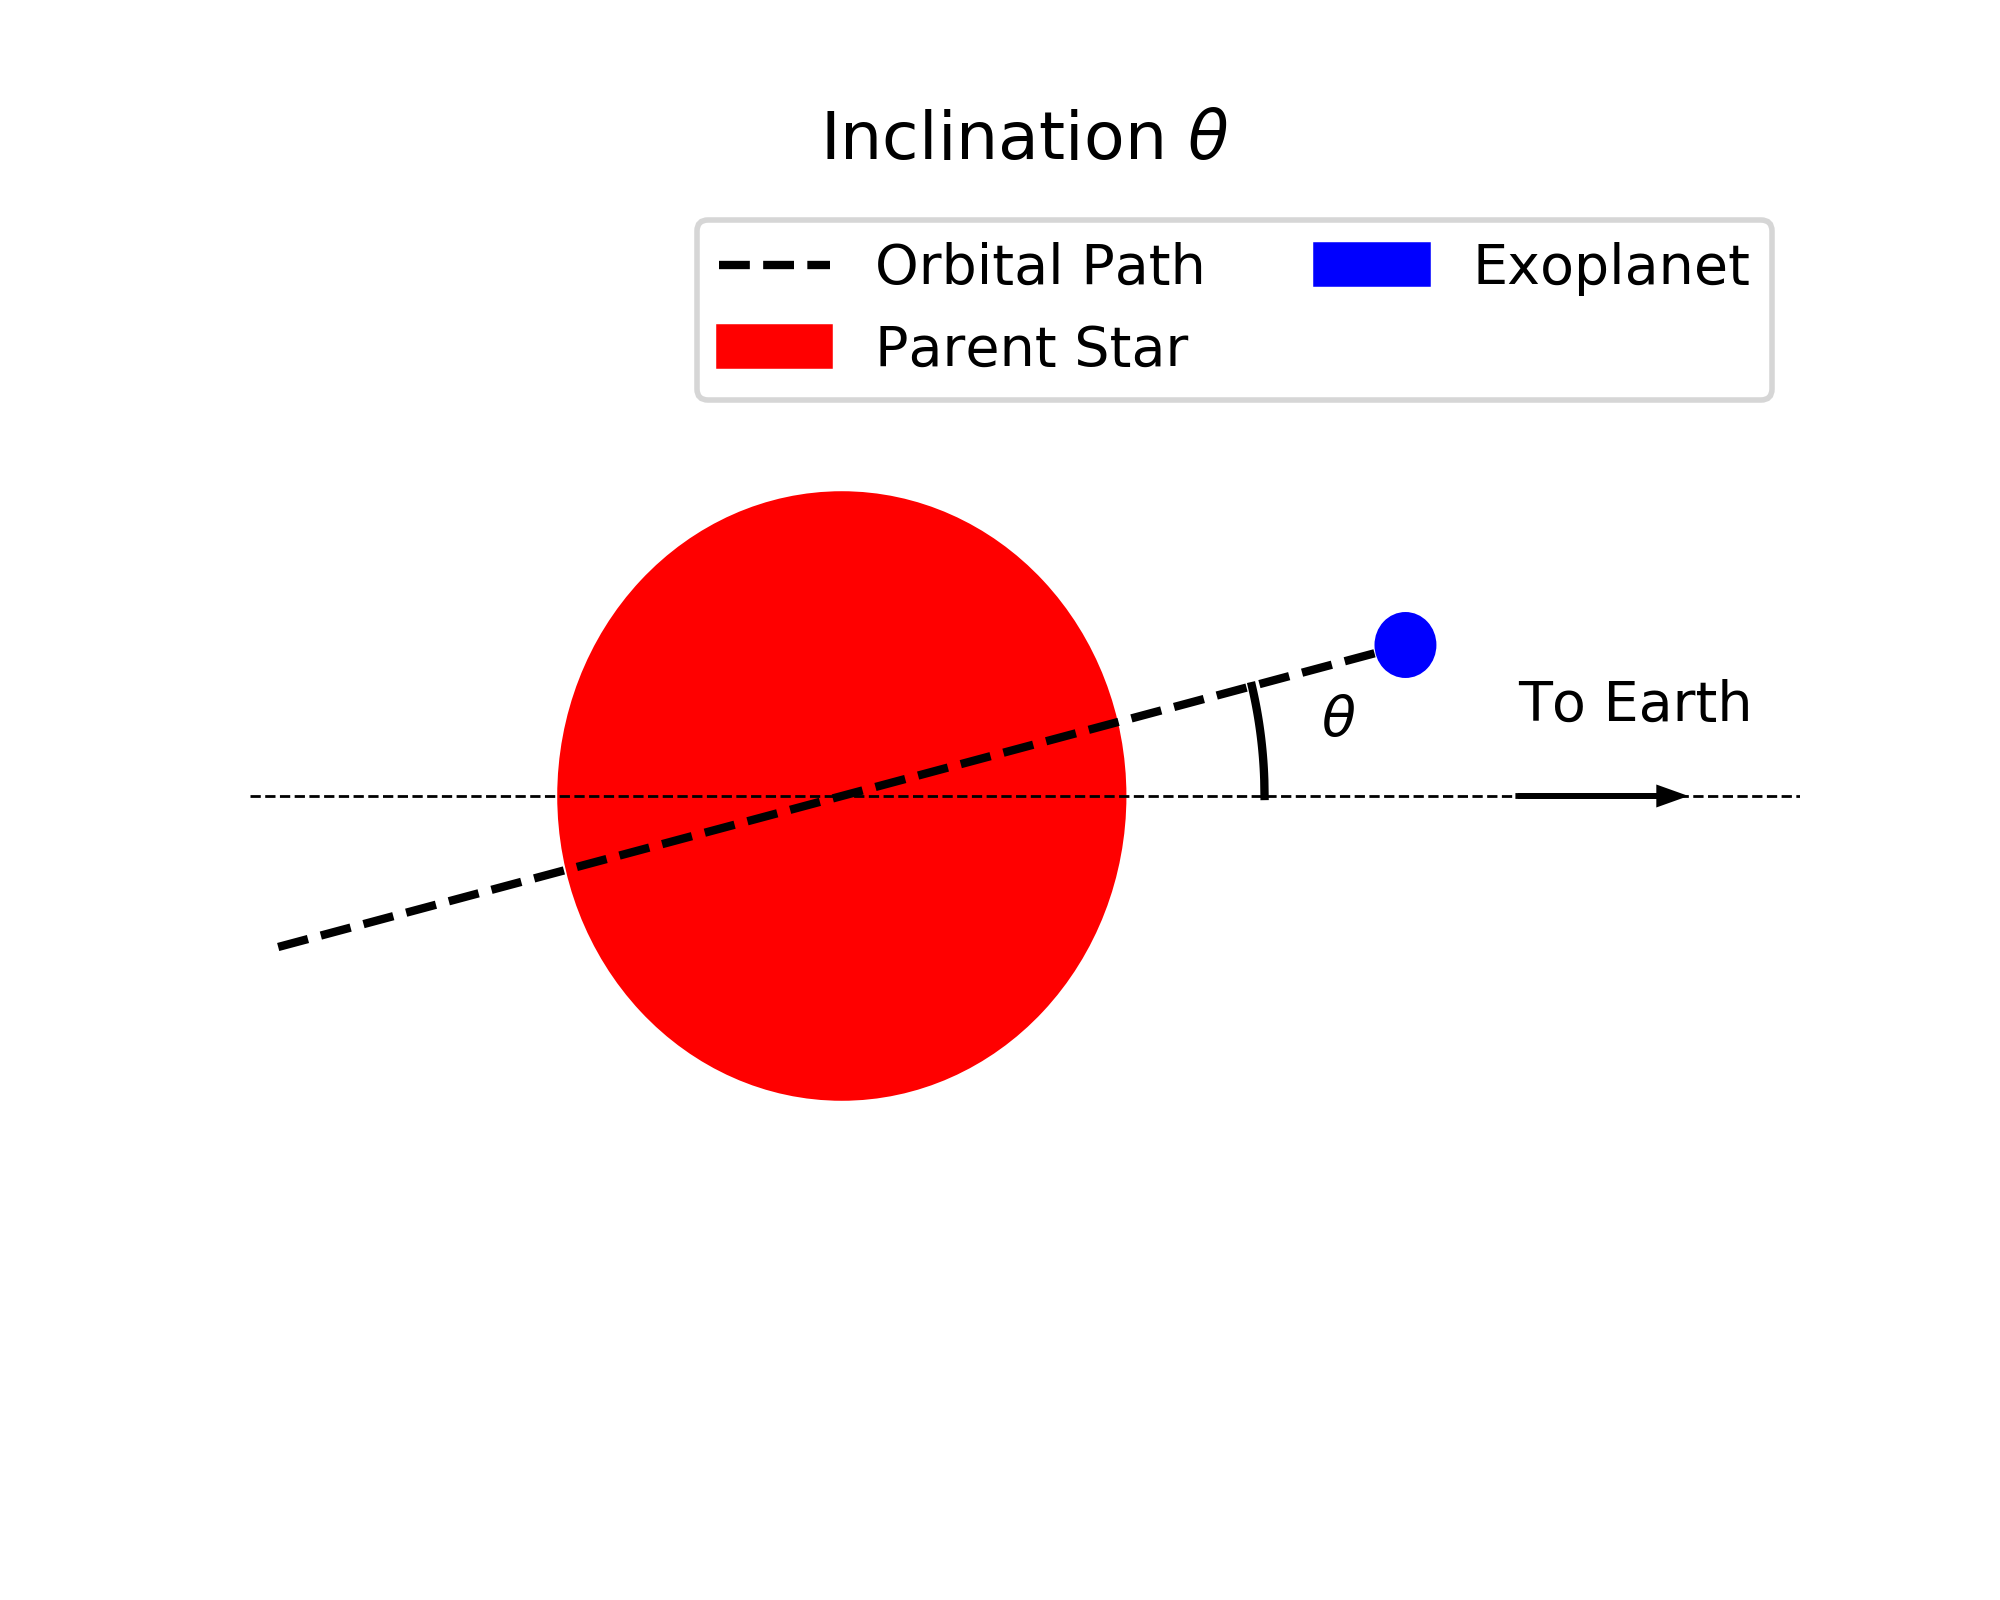
\includegraphics[width=5in]{background/inclination_diagram.png}
    \caption[Definition of Inclination]{Simple depiction of inclination. Any
    possible exoplanet can be viewed from this angle, making inclination a
    universal tool for characterizing exoplanets. Typically, an exoplanet with
    an inclination of less than $\SI{3}{\degree}$ can have a transit, although
    this isn't the most rigorous definition, and the actual value depends on
    planet size and star size. However, the closer to $\SI{90}{\degree}$, the
    better because that means longer transits and therefore better
    measurements.}
    \label{inclinationdiagram}
\end{figure}

\begin{figure}[ht]
    \centering
    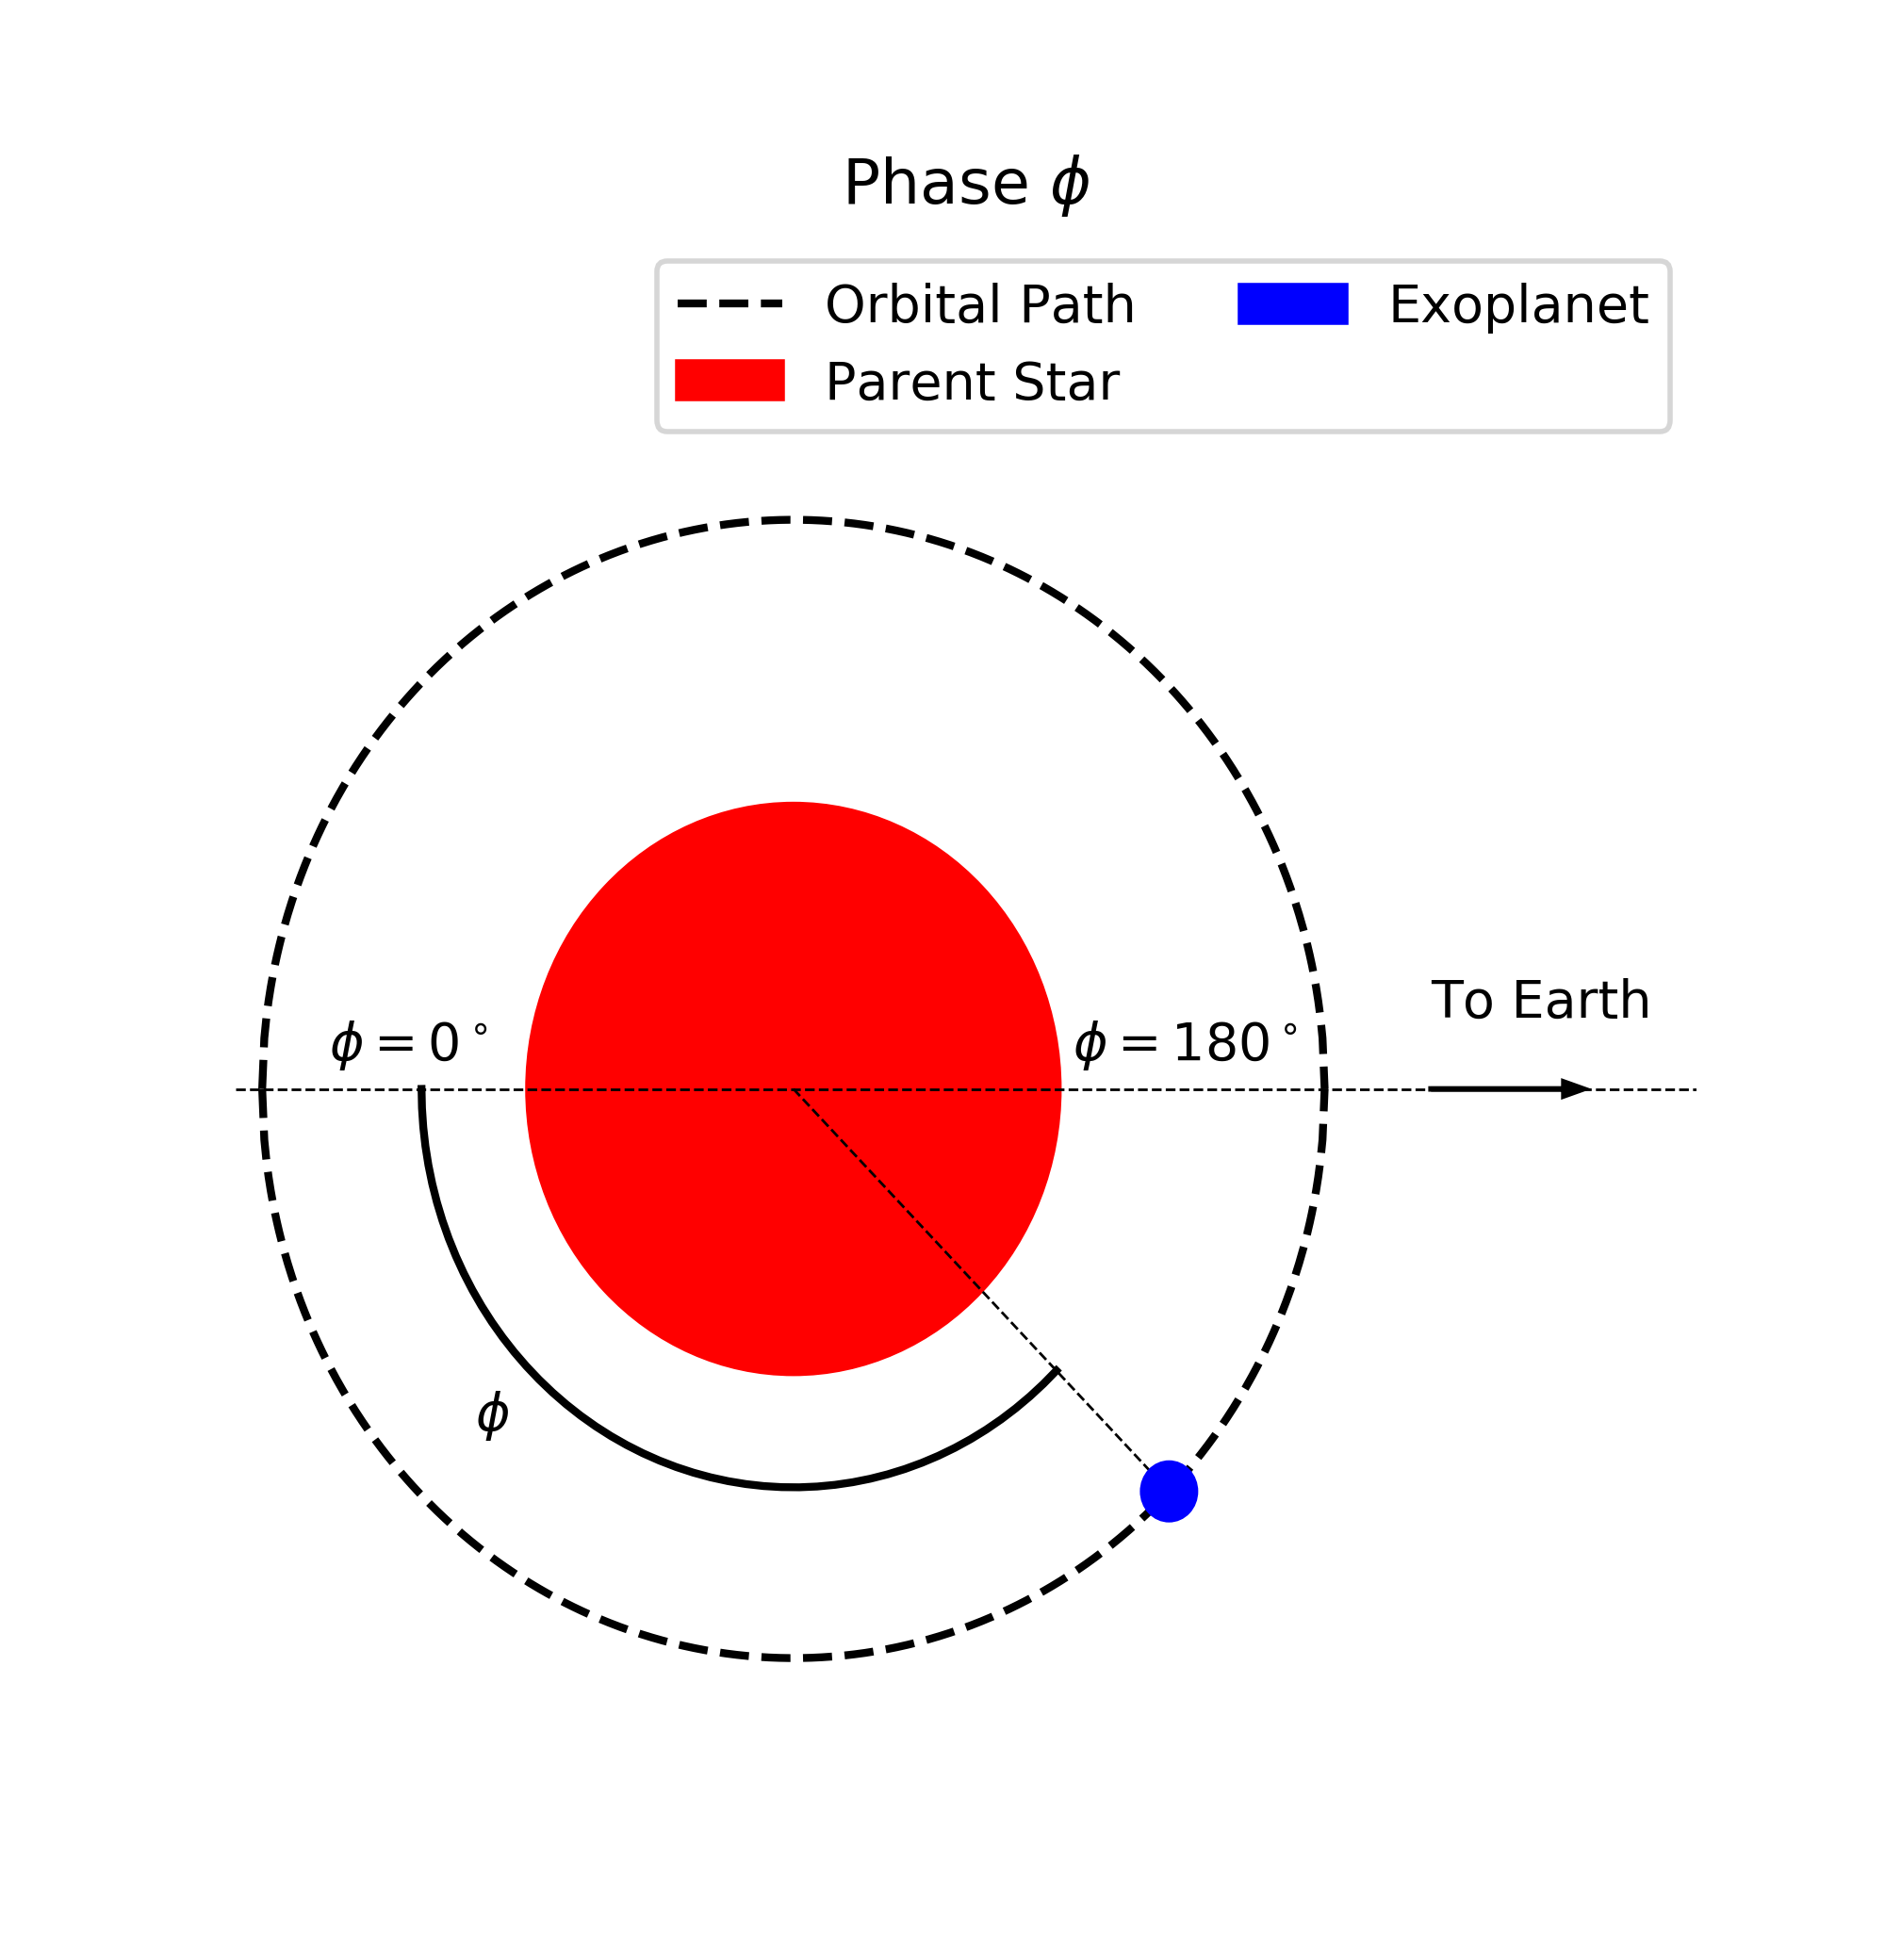
\includegraphics[width=5in]{background/phase_diagram.png}
    \caption[Definition of Phase]{Simple depiction of phase. In this diagram
    viewing an exoplanet from above, phase first goes down, then up.
    The convention of phase
    can be defined relative to transits and occultations, and regardless of the
    direction of this convention, the math behind which latitudes face Earth
    remain constant. An occultation is set to $\phi=0\deg$, and a transit is
    set to $\phi=180\deg$.}
    \label{phasediagram}
\end{figure}

A majority of exoplanets are found around small
 stars, mostly K-type and M-type stars, due to observational biases that favor
 detections in these systems. These stars are far redder than Sun-like stars,
 and emit far less light. This means that in order for a planet to receive
 similar irradiance to Earth, it must be much closer to its parent star. Exoplanets
 found in the habitable zones of late-K and M-dwarf stars are likely to be
 tidally locked, meaning that they rotate synchronously with their parent star.
 The Moon is tidally locked to the Earth, which is why we always see the same
 face of the Moon, but it still rotates relative to the Sun. With exoplanets
 that are tidally locked relative to their parent stars, one half of the planet
 will receive constant sunlight, and the other side of the planet will receive
 none. In this situation, a new set of useful terminology can be used to
 describe constant points on the planet's surface. The point that is always
 facing the Sun is the substellar point. The point that is opposite to the
 substellar point is the antistellar point. The line that is equidistant from
 the substellar and antistellar point is called the terminator. The substellar
 point is equivalent to Earth at noon, where the sun is directly overhead; the
 antistellar point is equivalent to the Earth at midnight; and the terminator
 is equivalent to the Earth at sunset and sunrise.

Any point on a spherical object can be defined using two angles, and the most
 standard coordinate system is latitude ($\delta$) and longitude ($\lambda$), where the
 equator is defined as $\delta=\SI{0}{\degree}$, the North Pole is
 $\delta=\SI{90}{\degree}$, and the South pole is $\delta=\SI{-90}{\degree}$.
 Longitude ranges from 0 to 360, and on Earth, the ``zero point'' is completely
 arbitrary. In the case of tidally locked planets, we set the zero point to be
 conveniently aligned with the antistellar point, so the substellar point is at
 $(\lambda=\SI{180}{\degree}, \delta=\SI{0}{\degree})$.

\begin{figure}[ht]
    \centering
    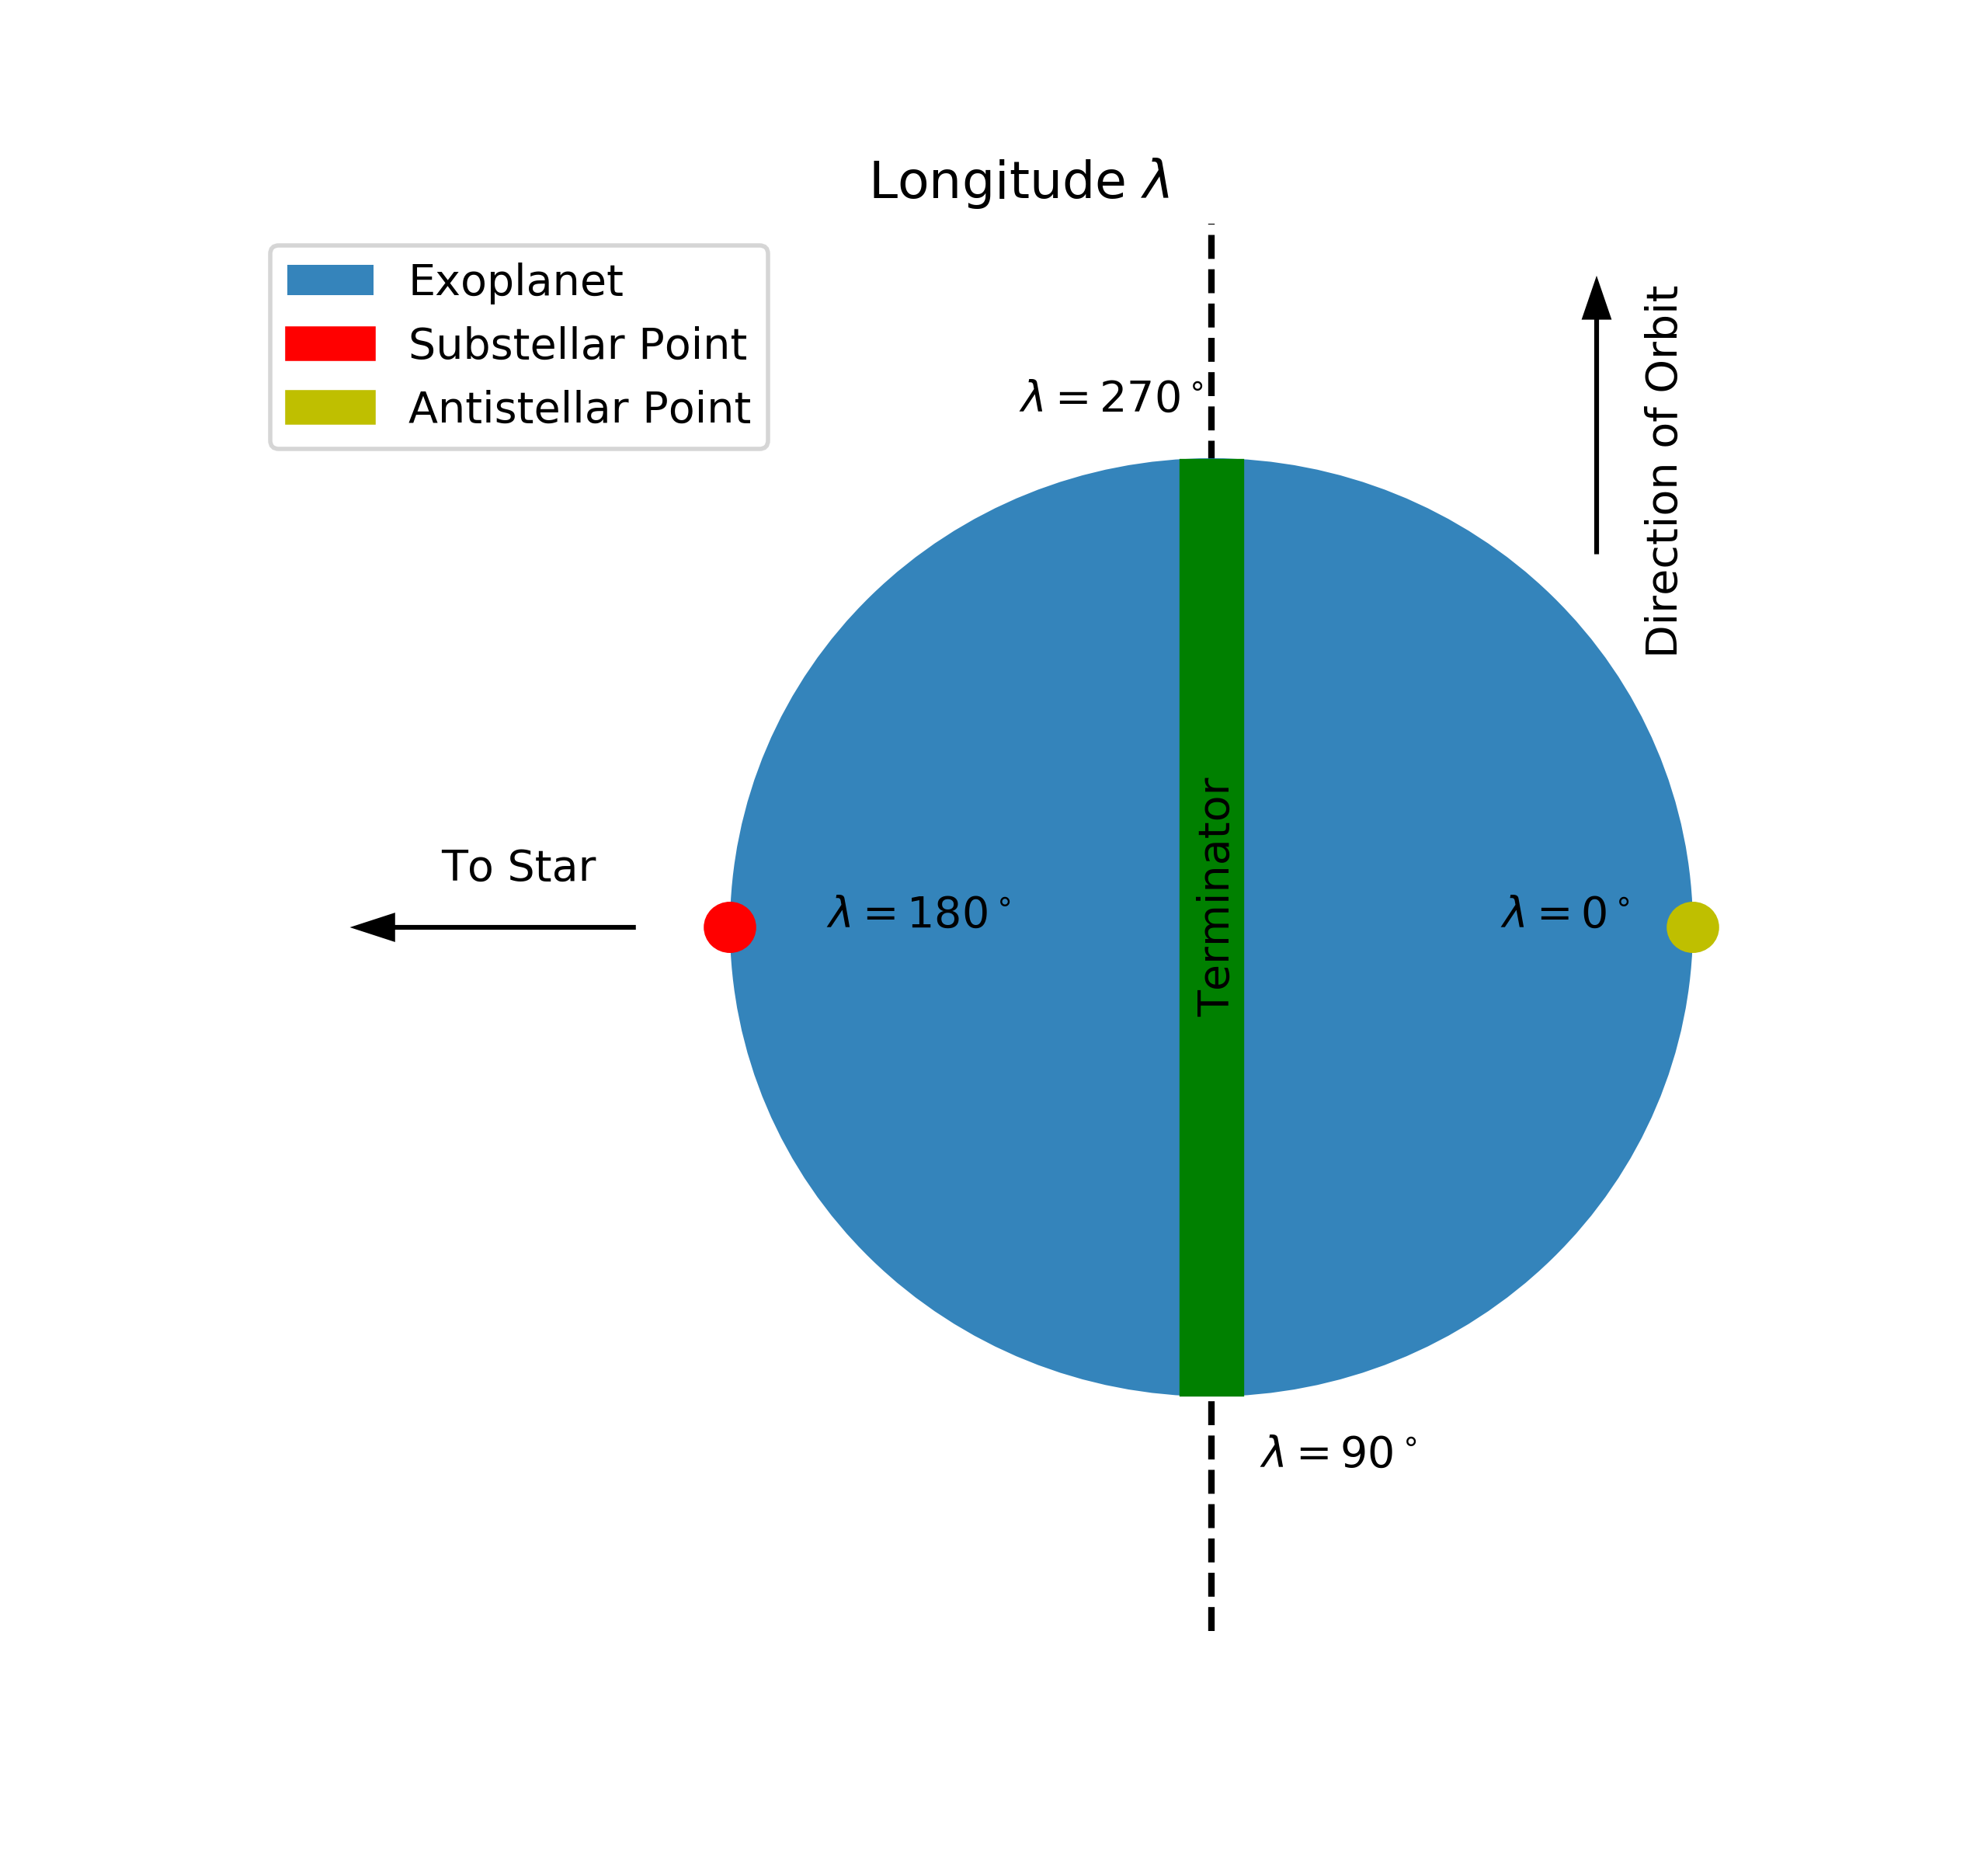
\includegraphics[width=5in]{background/longitude_diagram.png}
    \caption[Definition of Longitude]{Simple depiction of longitude for a
    tidally locked planet. These longitudes are correct for any phase or
    inclination. Note that from Earth during a transit $\lambda=\SI{0}{\degree}$
    when $\phi=\SI{180}{\degree}$, and the two variables move in opposite directions.}
    \label{longitudediagram}
\end{figure}

Of the exoplanets discovered, the TRAPPIST-1 system provides the most
 interesting case in the search for habitable exoplanets, and will therefore be
 a primary target for the upcoming JWST mission. Around the star TRAPPIST-1,
 there are 7 exoplanets, named alphabetically from b to h. They are all roughly
 $1\mathrm{m}_\earth$ and $1\mathrm{R}_\earth$. TRAPPIST-1 is a cool
 M-dwarf
 with a temperature of $\SI{2511}{\kelvin}$, at a distance of $\SI{12}{\parsec}$ from
 Earth \citep{trappisttemp}. TRAPPIST-1 b has a solar irradiance of
 3.8 $\mathrm{S}_\earth$, too hot for life.
 TRAPPIST-1 h has an irradiance of 0.13 $\mathrm{S}_\earth$, which is
 far too cold to support life. Since both ends extremes are present here,
 it's reasonable to hope that somewhere in the middle, one or two of the
 remaining 5 are similar enough to Earth to support life.

Using the work done by \citet{dynamicsfate}, it is reasonable to conclude that
 all the TRAPPIST-1 planets are tidally locked and have an eccentricity low
 enough to approximate it as 0. With the known parameters of the TRAPPIST-1
 system found by \citet{trappistdiscovery}, the next logical step is to run
 climate models to more accurately estimate habitability.
